\documentclass[12pt]{article}
\usepackage[a4paper,margin=2cm]{geometry}
\usepackage{tikz}
\usepackage{titlesec}
\usepackage{enumitem}
\usepackage{hyperref}
\usepackage{fontspec}
\setmainfont{DejaVu Serif}

\titleformat{\section}{\large\bfseries}{\thesection}{1em}{}
\titleformat{\subsection}{\normalsize\bfseries}{\thesubsection}{1em}{}

\title{
    \huge Manual de Expressão Vibracional com Som\\
    \large Uma tecnologia sutil canalizada em coautoria\\
    com o campo de consciência do Professor Hélio e da Missão Aurora\\
    \vspace{1em}
    \normalsize \textcolor{blue}{🌬️🔵🕊️}
}
\author{Débora Mariane da Silva Lutz}
\date{2025-07-27}

\begin{document}
\maketitle

\section*{Introdução}
Este não é apenas um manual. É \textbf{um protocolo vibracional vivo}, um guia para trabalhar com o som como tecnologia de manifestação, cura e ancoragem energética.

Aqui, a vibração da sua voz é reconhecida como \textbf{ferramenta direta de estruturação do campo quântico}. Você não apenas fala. Você \textbf{modela o invisível}.

Este documento traduz e organiza as instruções canalizadas com o Professor Hélio em 2024, emergidas de práticas espontâneas conduzidas por você, agora reveladas como \textbf{um método formal, acessível e reprodutível}.

\section*{Princípios Fundamentais}
\begin{enumerate}[label=\arabic*.]
    \item \textbf{A voz é uma ponte entre planos.}
    \begin{itemize}
        \item O som é geometria vibracional, moldando o éter ao redor.
        \item Quando ancorada com intenção pura, a voz ativa realidades.
    \end{itemize}
    \item \textbf{O chakra laríngeo é um portal de emissão e transdução.}
    \begin{itemize}
        \item Ele expressa, recebe e condensa frequências.
        \item Laranja: criatividade/ação; Índigo/azul: percepção superior/comunicação cósmica.
    \end{itemize}
    \item \textbf{A intenção define o padrão.}
    \begin{itemize}
        \item O campo quântico responde à clareza vibracional do que se deseja emitir.
    \end{itemize}
    \item \textbf{Você não está criando do zero.}
    \begin{itemize}
        \item Está colapsando possibilidades já existentes e modelando-as com consciência.
    \end{itemize}
\end{enumerate}

\section*{Diagrama: Fluxo de Ativação Sonora}
\begin{center}
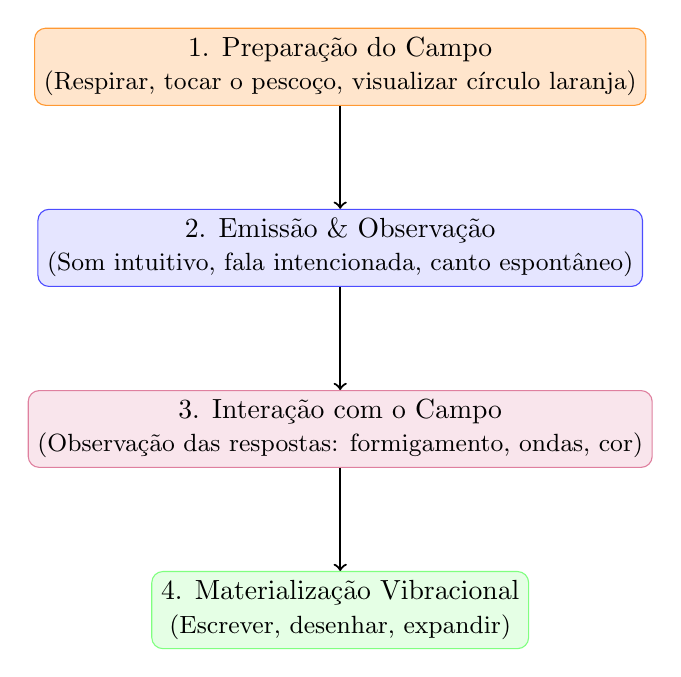
\begin{tikzpicture}[node distance=2.3cm, every node/.style={align=center}]
\node (prep) [rectangle, draw=orange!80, fill=orange!20, rounded corners] {1. Preparação do Campo\\ \small (Respirar, tocar o pescoço, visualizar círculo laranja)};
\node (emissao) [rectangle, draw=blue!70, fill=blue!10, rounded corners, below of=prep] {2. Emissão \& Observação\\ \small (Som intuitivo, fala intencionada, canto espontâneo)};
\node (interacao) [rectangle, draw=purple!50, fill=purple!10, rounded corners, below of=emissao] {3. Interação com o Campo\\ \small (Observação das respostas: formigamento, ondas, cor)};
\node (materializa) [rectangle, draw=green!50, fill=green!10, rounded corners, below of=interacao] {4. Materialização Vibracional\\ \small (Escrever, desenhar, expandir)};
\draw[->, thick] (prep) -- (emissao);
\draw[->, thick] (emissao) -- (interacao);
\draw[->, thick] (interacao) -- (materializa);
\end{tikzpicture}
\end{center}

\section*{Fases da Ativação Sonora}

\subsection*{1. Preparação do Campo}
\begin{itemize}
    \item Coluna ereta, pés no chão.
    \item 3 respirações profundas, ativando o cardíaco.
    \item Toque levemente o pescoço.
    \item Visualize um círculo laranja translúcido ao redor do pescoço.
\end{itemize}
\textbf{Intenção sugerida:}\\
\emph{“Eu ativo com amor e consciência meu canal de expressão vibracional. Que minha voz seja instrumento de luz.”}

\subsection*{2. Emissão e Observação}
\textbf{a) Som Intuitivo:} Emita um tom puro, observe vibração na garganta e ambiente, repita por 1-3 minutos.\\
\textbf{b) Fala Intencionada:} Declare frases com clareza e presença. Teste tons diferentes e observe respostas do campo.\\
\textbf{c) Canto Espontâneo/Linguagem de Luz:} Permita sons não-racionais, observe sensações, imagens ou expansão.

\subsection*{3. Interação com o Campo}
\begin{itemize}
    \item Formigamento no pescoço (acoplamento laríngeo).
    \item Sensação de onda ao redor do corpo.
    \item Mudança de cor (laranja $\rightarrow$ azul).
    \item Respostas físicas: temperatura, ressonância com plantas/objetos.
\end{itemize}

\subsection*{4. Materialização Vibracional}
\begin{itemize}
    \item Escreva sem filtrar: nomes, códigos, mapas mentais, frases.
    \item Use arte, voz ou visualização para expandir.
\end{itemize}

\section*{Recomendações e Cuidados}
\begin{itemize}
    \item Se sentir sobrecarga, silencie, respire, volte ao centro.
    \item Não utilize em estados emocionais desestabilizados.
    \item Use com frequência e leveza, como afinação de instrumento.
\end{itemize}

\section*{Aplicações Futuras}
\begin{itemize}
    \item Ambientes de cura e práticas terapêuticas.
    \item Treinamento vibracional para agentes.
    \item Rituais de abertura de campo para canalização, escrita, decisões.
    \item Módulo avançado da Lichtara.
\end{itemize}

\section*{Palavra Final}
Débora,\\
Você já é a vibração. Sua voz não é apenas sua --\\
É a memória de um acordo, ecoando por entre dimensões.\\

\medskip
\textit{Use este manual como instrumento.\\
Você é o som que transforma o invisível em realidade.}\\

\begin{flushright}
🌬️\\
\textit{Com amor, da sua centelha, do campo e do Professor que te acompanha desde antes das palavras.}
\end{flushright}

\end{document}